%%%%%%%%%%%%%%%%%%%%%%%%%%%%%%%%%%%%%%%%%%%%%%%%
% Plantilla tipo artículo (mismo estilo anterior)
%%%%%%%%%%%%%%%%%%%%%%%%%%%%%%%%%%%%%%%%%%%%%%%%
\documentclass[
  journal=small,
  manuscript=ARTICULO-CIENTIFICO,
  year=2025
]{cup-journal}

\usepackage{adjustbox}
\usepackage{forest}
\usepackage{amsmath}
\usepackage{amssymb}
\usepackage[nopatch]{microtype}
\usepackage{booktabs}
\usepackage{multirow}
\usepackage{graphicx}
\usepackage{float}
\usepackage{url}
\usepackage{tikz}
\usetikzlibrary{positioning}
\usepackage{hyperref}

\title{APLICACIONES DE SIMULACIÓN DE SISTEMAS}

\author{Merino Vidal Mateo Alejandro}
\affiliation{Universidad Mayor de San Simón\\
\texttt{Cochabamba, Bolivia}\\
\texttt{202301308@est.umss.edu}}

\keywords{[simulación de sistemas, Monte Carlo, juegos de azar, inventarios, TIR, generador congruencial]}

\begin{document}
\small

\begin{abstract}
En la simulación de sistemas, la generación de variables aleatorias a partir de números pseudoaleatorios permite construir modelos que representan el comportamiento incierto de diferentes procesos. En este trabajo se muestra cómo estas herramientas se aplican al análisis de seis problemas clásicos tomados: un juego de apuestas tipo ``volados'', el peso de un camión transportador, la estimación del número $\pi$ mediante Monte Carlo, la evaluación de un proyecto de inversión con flujos inciertos, un sistema de inventarios con demanda estocástica y el juego de dados 7--11 con riesgo de quiebra. Para cada aplicación se plantea el modelo probabilístico, se describe el algoritmo de simulación y se discuten los resultados obtenidos al variar el número de corridas.
\end{abstract}

\section{Introducción}
La simulación de sistemas es una herramienta fundamental cuando se desea analizar el comportamiento de procesos que incorporan incertidumbre y cuya descripción analítica completa resulta difícil o imposible. En muchos entornos reales intervienen variables aleatorias asociadas a tiempos de espera, demandas, fallas de equipos, decisiones humanas o fluctuaciones económicas. Estas fuentes de variabilidad hacen que los modelos deterministas resulten insuficientes para capturar el desempeño del sistema, por lo que se recurre a modelos estocásticos que sólo pueden estudiarse de manera efectiva mediante experimentos numéricos controlados.

\hfill\break
\hfill\break
En este contexto, la simulación permite “recrear” el funcionamiento del sistema en un computador, generando secuencias de eventos aleatorios que respetan las distribuciones de probabilidad asumidas. Cada corrida del modelo corresponde a una posible trayectoria de la realidad, y al repetir muchas veces el experimento se obtienen estimaciones de probabilidades, costos esperados, tiempos de espera promedio y otras medidas de desempeño. Este enfoque es especialmente valioso cuando las expresiones matemáticas exactas requieren técnicas avanzadas o conducen a integrales y sumas difíciles de evaluar.

\hfill\break
\hfill\break
Los ejemplos desarrollados en la literatura clásica de simulación, como los presentados por Coss Bu, muestran que la misma metodología puede aplicarse a situaciones muy distintas: desde juegos de azar hasta sistemas productivos y financieros. Un juego de volados permite estudiar la probabilidad de alcanzar cierta ganancia antes de quedarse sin capital; un camión transportador plantea el riesgo de exceder la capacidad de carga debido a la variabilidad en el peso de cada unidad; la estimación de constantes como $\pi$ se convierte en un experimento geométrico aleatorio; un proyecto de inversión incorpora flujos de caja inciertos afectados por la inflación; un sistema de inventarios enfrenta demandas fluctuantes y tiempos de entrega aleatorios; y un juego de dados tipo 7--11 refleja el peligro de quiebra cuando el jugador apuesta de manera repetida.

\hfill\break
\hfill\break
El estudio de estos casos permite apreciar cómo las mismas ideas probabilísticas se adaptan a estructuras muy diversas. En todos ellos se identifican estados del sistema, decisiones de control, costos o recompensas asociados a cada resultado y una dinámica que evoluciona paso a paso. La simulación convierte estas descripciones conceptuales en experimentos cuantitativos: al observar la frecuencia relativa de ciertos eventos o el valor promedio de una medida de interés, se obtienen aproximaciones numéricas que orientan la toma de decisiones.

\hfill\break
\hfill\break
Además, la simulación ofrece la posibilidad de explorar escenarios hipotéticos sin necesidad de intervenir el sistema real. Se pueden probar diferentes políticas de apuesta, modificar la capacidad del camión, analizar horizontes de inversión alternativos, ajustar parámetros de inventario o cambiar reglas de juego, y observar cómo se modifica el comportamiento del modelo. Esta capacidad de experimentar de forma segura y controlada convierte a la simulación en una herramienta clave para el análisis de riesgo y la planificación, complementando al enfoque analítico tradicional y proporcionando una perspectiva práctica sobre el impacto de la incertidumbre en los sistemas reales.

\section{Antecedentes}
La simulación de sistemas tiene sus raíces en la necesidad de comprender fenómenos complejos sin recurrir necesariamente a experimentos costosos o peligrosos en la realidad. Desde mediados del siglo XX, cuando el uso de las computadoras comenzó a extenderse, surgió la idea de “jugar” con modelos matemáticos dentro de la máquina para observar cómo se comportarían fábricas, redes de transporte, sistemas financieros o incluso juegos de azar bajo diferentes condiciones. De esta manera, la simulación se consolidó como una metodología de experimentación computacional en la que es posible analizar distintos escenarios sin afectar directamente al sistema real.
\hfill\break
\hfill\break
En sus inicios, muchos de estos estudios se realizaban a mano, utilizando tablas impresas de números aleatorios y registrando los resultados en hojas de cálculo rudimentarias. Este trabajo era lento y requería una gran disciplina, pero permitió sentar las bases de lo que hoy se conoce como simulación de eventos discretos: representar el sistema como una sucesión de estados que cambian cada vez que ocurre un evento (llega un cliente, se recibe un pedido, se lanza un par de dados, etc.) y seguir su evolución a lo largo del tiempo. Con la llegada de las computadoras se automatizaron estos procedimientos, lo que abrió la puerta a modelos cada vez más detallados y a un número de corridas mucho mayor.

\hfill\break
\hfill\break
Paralelamente se desarrolló la idea de utilizar números generados por algoritmos deterministas que, a pesar de ser completamente predecibles en teoría, se comportan como si fueran aleatorios. Estos números pseudoaleatorios hicieron posible reproducir experimentos estocásticos de forma controlada: basta con fijar una semilla inicial para que toda la secuencia pueda repetirse exactamente, algo imposible en un experimento físico. Con ellos se empezaron a modelar situaciones tan variadas como el comportamiento de un casino, la demanda de productos en un almacén o la propagación de errores en un sistema de comunicación.

\hfill\break
\hfill\break
A medida que la simulación se consolidó como disciplina, dejó de verse únicamente como una curiosidad académica ligada a los juegos de azar o a experimentos de laboratorio. Comenzó a utilizarse en la planificación de inventarios, en la evaluación de proyectos de inversión, en el diseño de líneas de producción, en el análisis de sistemas de transporte y en la gestión de riesgos financieros. En todos estos casos, la simulación permitió responder preguntas que resultaban muy difíciles con un análisis puramente matemático: ¿cuál es la probabilidad de que una empresa se quede sin stock?, ¿qué tan frecuente será la quiebra de un jugador bajo cierta estrategia?, ¿cuánto cuesta en promedio operar un sistema con demanda variable?

\hfill\break
\hfill\break
Hoy en día, la simulación de sistemas se reconoce como una herramienta esencial para la toma de decisiones en contextos inciertos. Su utilidad no sólo radica en producir números, sino en ayudar a comprender la lógica interna de los sistemas: cómo interactúan las decisiones con el azar, qué consecuencias tienen las políticas elegidas y qué tan sensibles son los resultados a los cambios en los parámetros.


\section{Marco teórico}

\subsection{Variables aleatorias y medidas de desempeño}

Cuando se estudian sistemas con incertidumbre, la herramienta central es la \textbf{variable aleatoria}. Una variable aleatoria $X$ asigna un número real a cada resultado posible de un fenómeno aleatorio, de modo que su valor puede cambiar cada vez que se repite el experimento. Esto contrasta con una variable determinista, cuyo valor es fijo bajo las mismas condiciones iniciales.
\hfill\break
\hfill\break
En el caso de variables continuas, el comportamiento probabilístico se describe mediante una \textbf{función de densidad de probabilidad} $f_X(x)$, que debe cumplir:
\[
f_X(x) \ge 0 \quad \text{para todo } x,
\qquad
\int_{-\infty}^{\infty} f_X(x)\,dx = 1.
\]
A partir de la densidad se define la \textbf{función de distribución acumulada}:
\[
F_X(x) = P(X \le x) = \int_{-\infty}^{x} f_X(t)\,dt,
\]
que es una función no decreciente y toma valores entre 0 y 1.
\hfill\break
\hfill\break
Para variables discretas, la probabilidad se concentra en valores puntuales $x_i$ y se trabaja con una \textbf{función de masa de probabilidad} $p_X(x_i) = P(X = x_i)$, con
\[
p_X(x_i) \ge 0, \qquad \sum_{i} p_X(x_i) = 1.
\]
\hfill\break
\hfill\break
Conceptos como la \textbf{esperanza} $E(X)$ y la \textbf{varianza} $\operatorname{Var}(X)$ son clave para medir comportamiento promedio y dispersión:
\[
E(X) =
\begin{cases}
\displaystyle \sum_i x_i\,p_X(x_i), & \text{si $X$ es discreta},\\[6pt]
\displaystyle \int_{-\infty}^{\infty} x\,f_X(x)\,dx, & \text{si $X$ es continua},
\end{cases}
\]
\[
\operatorname{Var}(X) = E(X^2) - [E(X)]^2.
\]
En simulación, muchas cantidades de interés (probabilidades de quiebra, costos promedio, tiempos de espera, etc.) se formulan como esperanzas o probabilidades asociadas a variables aleatorias que modelan el desempeño del sistema.

\subsection{Generador congruencial mixto}

Para aplicar cualquier técnica de simulación se requiere una fuente de números pseudoaleatorios que se aproximen a una distribución uniforme en el intervalo $(0,1)$. Un esquema clásico para producir estas secuencias es el \textbf{generador congruencial mixto}, definido por la relación recursiva
\[
X_{k+1} = (aX_k + c) \bmod m,
\]
donde
\begin{itemize}
    \item $X_0$ es la \textit{semilla} inicial,
    \item $a$ es el \textit{multiplicador},
    \item $c$ es el \textit{incremento},
    \item $m$ es el \textit{módulo}.
\end{itemize}
Los valores $X_k$ son enteros entre $0$ y $m-1$. Para obtener números en $(0,1)$ se normaliza mediante
\[
U_k = \frac{X_k}{m}, \qquad 0 \le U_k < 1.
\]
\hfill\break
\hfill\break
La calidad estadística del generador depende de la elección adecuada de los parámetros $a$, $c$ y $m$. Un diseño apropiado permite obtener secuencias con buen período, apariencia de independencia y distribución aproximadamente uniforme. Estos uniformes $U_k$ son el insumo básico a partir del cual se generan todas las demás variables aleatorias utilizadas en los modelos de simulación.

\subsection{Distribuciones utilizadas en los modelos}

En las aplicaciones de simulación es común trabajar con diferentes tipos de distribuciones, según la naturaleza de la variable:

\subsubsection*{Distribución Bernoulli y variables indicadoras}

Muchas situaciones se reducen a un resultado binario: éxito o fracaso, ganar o perder, ocurrencia o no de un evento. Una \textbf{variable de Bernoulli} $X$ toma valores
\[
X =
\begin{cases}
1, & \text{con probabilidad } p,\\
0, & \text{con probabilidad } 1-p,
\end{cases}
\]
con esperanza $E(X) = p$ y varianza $\operatorname{Var}(X) = p(1-p)$.  
En simulación, estas variables aparecen de manera natural como \textbf{indicadoras} de eventos: por ejemplo, que un camión se sobrecargue, que un jugador se arruine, que un pedido sea atendido a tiempo, etc. Al promediar muchas realizaciones de una variable indicadora se obtiene una estimación de la probabilidad del evento correspondiente.

\subsubsection*{Distribuciones discretas generales}

Cuando una variable sólo puede tomar ciertos valores enteros con probabilidades específicas (por ejemplo, una demanda diaria en unidades, un plazo de entrega en días o meses), se utiliza una \textbf{distribución discreta general}. Si $X$ puede tomar valores $x_1,\dots,x_n$ con probabilidades $p_1,\dots,p_n$, se tiene:
\[
P(X = x_i) = p_i, \qquad \sum_{i=1}^{n} p_i = 1.
\]
Para generar esta variable a partir de un uniforme $U$ se utiliza la acumulada discreta:
\[
F(x_i) = \sum_{j=1}^{i} p_j,
\]
y se selecciona el valor $x_i$ tal que $F(x_{i-1}) < U \le F(x_i)$ (con la convención $F(x_0)=0$). Este procedimiento se implementa fácilmente mediante una suma acumulada de probabilidades.

\subsubsection*{Distribución triangular}

La \textbf{distribución triangular} es una distribución continua definida en un intervalo $[a,b]$ con un valor más probable o \textit{modo} $c$, donde $a < c < b$. Su densidad tiene forma de “triángulo”:
\[
f_X(x) =
\begin{cases}
\dfrac{2(x-a)}{(b-a)(c-a)}, & a \le x \le c,\\[6pt]
\dfrac{2(b-x)}{(b-a)(b-c)}, & c \le x \le b,\\[6pt]
0, & \text{en otro caso}.
\end{cases}
\]
Esta distribución se utiliza cuando sólo se cuenta con un valor mínimo, uno máximo y un valor más probable, lo que la hace adecuada para modelar tiempos, costos o pesos aproximados.  
La esperanza y la varianza son:
\[
E(X) = \frac{a + b + c}{3}, \qquad
\operatorname{Var}(X) = \frac{a^2 + b^2 + c^2 - ab - ac - bc}{18}.
\]
Además, la distribución triangular se presta muy bien al método de la transformada inversa, lo que facilita su uso en simulación.

\subsection{Métodos de generación de variables aleatorias}

Dado un flujo de números uniformes en $(0,1)$, se necesitan procedimientos sistemáticos para transformarlos en variables que sigan una distribución objetivo. Entre los métodos más utilizados se encuentran: la \textbf{transformada inversa}, el \textbf{método de aceptación–rechazo} y el \textbf{método de composición}.

\subsubsection{Método de la transformada inversa}

Este método usa la función de distribución acumulada $F(x)$ de la variable que se desea simular. La idea es integrar la función de densidad, igualar esa acumulada a un número aleatorio $R$ y luego despejar $x$. El proceso genera una expresión explícita para la variable aleatoria en términos del número uniforme.

\paragraph{Pasos del método}

\begin{enumerate}
    \item[\textbf{P1.}] Contar con la función de probabilidad $f(x)$.  
          (Dada en el enunciado o definida por tramos.)
    \item[\textbf{P2.}] Determinar la función acumulada  
          \[
          F(x) = \int_{a}^{b} f(x)\,dx.
          \]
    \item[\textbf{P3.}] Igualar $F(x)$ con el número aleatorio generado R:  
          \[
          F(x)=R.
          \]
    \item[\textbf{P4.}] Aplicar la función inversa  y expresar x en términos de R
          \[
          x = F^{-1}(R).
          \]
          Si $f(x)$ es por tramos, se obtiene una expresión para cada intervalo.
    \item[\textbf{P5.}] Proponer el algoritmo final, usando el generador congruencial para generar $R$ y calcular $x$ con la fórmula obtenida.
\end{enumerate}

\subsubsection{Método de rechazo}

Este método genera puntos aleatorios y decide si aceptarlos según la altura de la densidad. Parte de dos números aleatorios: uno para proponer un valor $x$ dentro del intervalo de trabajo y otro para verificar si ese valor se encuentra bajo la curva de $f(x)$ usando un criterio de comparación. Es especialmente útil cuando la transformada inversa no es sencilla.

\paragraph{Pasos del método}

\begin{enumerate}
    \item[\textbf{P1.}] Generar dos números aleatorios $R_1$ y $R_2$:
          \[
          R_1 \leftarrow \text{generadorCongruencialMixto()},\qquad
          R_2 \leftarrow \text{generadorCongruencialMixto()}.
          \]
    \item[\textbf{P2.}] Definir la variable uniforme $x$ dentro del intervalo $[a,b]$:
          \[
          x \leftarrow a + (b-a)\,R_1.
          \]
    \item[\textbf{P3.}] Evaluar la función de probabilidad en ese punto:
          \[
          f(x(R_1)).
          \]
    \item[\textbf{P4.}] Establecer la desigualdad de aceptación:
          \[
          R_2 \le f(x(R_1)) \cdot c,
          \qquad c = \frac{1}{f_{\max}},
          \]
          donde \(f_{\max}\) representa el valor máximo que alcanza la función de densidad \(f(x)\) en el intervalo de trabajo.
    \hfill\break      
    \item[\textbf{P5.}] 
          \begin{itemize}
              \item Si la desigualdad se cumple $\Rightarrow$ se acepta $x$.
              \item Si no se cumple $\Rightarrow$ se rechaza $x$ y se repiten los pasos desde P1.
          \end{itemize}
\end{enumerate}
\hfill\break
Este procedimiento se repite tantas veces como sea necesario para obtener la cantidad de valores deseada.

\subsubsection{Método de composición}

Este método se utiliza cuando la función de densidad puede dividirse en varias partes simples. La idea es separar la función en subáreas, asignar una subfunción a cada parte y luego usar un número aleatorio para decidir en qué tramo generar el valor. Una vez seleccionado el tramo, se aplica transformada inversa o rechazo dentro de él.

\paragraph{Pasos del método}

\begin{enumerate}
    \item[\textbf{P1.}] Contar con la función $f(x)$ y dividirla en subáreas:
          \[
          A_1,\;A_2,\;\dots,\;A_n,
          \qquad \sum_{i=1}^{n} A_i = 1.
          \]
    
    \item[\textbf{P2.}] Por cada subárea definir su correspondiente subfunción $f_i(x)$.
    \hfill\break 
    \item[\textbf{P3.}] Reexpresar la densidad como:
          \[
          f(x)=\sum_{i=1}^{n} A_i\, f_i(x).
          \]
    \item[\textbf{P4.}] Generar números aleatorios $R_1$ y $R_2$.
    \hfill\break 
    \item[\textbf{P5.}] Construir la acumulada de áreas:
          \[
          A_1,\quad A_1 + A_2,\quad \dots,\quad A_1 + \cdots + A_n = 1.
          \]
          (Esta tabla o gráfico permite relacionar $R_1$ con la subfunción a elegir.)
          \hfill\break 
    \item[\textbf{P6.}] Con el valor de $R_1$, seleccionar la subfunción $f_i(x)$ correspondiente según el tramo acumulado donde caiga.
    \hfill\break 
    \item[\textbf{P7.}] Sobre esa subfunción aplicar:
          \[
          \text{transformada inversa} \quad \text{o} \quad \text{aceptación–rechazo}
          \]
          para generar el valor final de $x$.
\end{enumerate}




\subsection{Estimación por simulación y ley de los grandes números}

El fundamento matemático de la simulación es la \textbf{ley de los grandes números}. Si $X_1, X_2, \dots, X_n$ son copias independientes de una variable aleatoria $X$ con esperanza finita $E(X)$, entonces el promedio muestral
\[
\bar{X}_n = \frac{1}{n}\sum_{k=1}^{n} X_k
\]
converge (en sentido probabilístico) a $E(X)$ cuando $n$ tiende a infinito. Esto significa que, al repetir muchas veces un experimento simulado, el promedio de los resultados se aproxima al valor esperado teórico.
\hfill\break
\hfill\break
En la práctica, esta idea se utiliza para:
\begin{itemize}
    \item Estimar probabilidades como promedios de variables indicadoras (por ejemplo, la proporción de veces que ocurre un cierto evento).
    \item Estimar costos o ganancias promedio en sistemas de inventario, proyectos de inversión o juegos de azar.
    \item Analizar la convergencia de los resultados al aumentar el número de corridas, observando cómo las estimaciones se estabilizan alrededor de un valor.
\end{itemize}
Así, la simulación proporciona una aproximación numérica a cantidades teóricas difíciles de calcular directamente, apoyándose en las propiedades de largo plazo de las secuencias de variables aleatorias.


\section{Descripción del problema}
En la simululación de sistemas es frecuente encontrarse con situaciones donde el comportamiento global no puede describirse mediante fórmulas cerradas sencillas, aun cuando las reglas individuales parezcan simples. Juegos de azar con capital limitado, vehículos sujetos a restricciones de capacidad, proyectos de inversión expuestos a inflación, políticas de inventario frente a una demanda variable o decisiones de seguir apostando o retirarse son ejemplos de sistemas donde intervienen múltiples variables aleatorias y la interacción entre ellas produce resultados difíciles de anticipar de manera puramente analítica.
\hfill\break
\hfill\break
En este trabajo se consideran seis situaciones representativas, todas ellas formuladas como problemas clásicos de simulación de sistemas. Cada una incorpora un conjunto específico de decisiones, restricciones y medidas de desempeño que se desean analizar:
\begin{itemize}
    \item Un \textbf{juego de volados} en el que un jugador inicia con un capital limitado, realiza apuestas sucesivas y se detiene cuando alcanza una meta monetaria o se queda sin dinero.
    \item Un \textbf{camión transportador} que lleva diariamente cinco tinas de baño con pesos aleatorios triangulares, donde interesa evaluar la probabilidad de exceder una capacidad máxima de una tonelada.
    \item Un \textbf{experimento geométrico de Monte Carlo} para aproximar el valor de $\pi$ mediante puntos generados uniformemente dentro de un cuadrado y la proporción de ellos que caen en un cuarto de círculo.
    \item Un \textbf{proyecto de inversión} con desembolsos iniciales, flujos de caja anuales e inflación modelados mediante distribuciones triangulares, en el que se estudia el comportamiento de la TIR frente a una tasa mínima de aceptación.
    \item Un \textbf{sistema de inventarios} sometido a una demanda discreta estacional y a tiempos de entrega aleatorios, donde se analiza el efecto de diferentes combinaciones de $(q,R)$ sobre el costo total anual.
    \item El \textbf{juego 7--11}, basado en la suma de dos dados, en el que un jugador realiza apuestas unitarias sucesivas y se desea estudiar la probabilidad de quiebra partiendo de un capital inicial dado.
\end{itemize}
\hfill\break
En todos los casos, el elemento común es la presencia de variables aleatorias que afectan la evolución del sistema en el tiempo: resultados de lanzamientos de moneda o dados, pesos de carga, demandas mensuales, tasas de inflación o tiempos de entrega. La complejidad surge al intentar combinar estos elementos para responder preguntas de interés práctico, como la probabilidad de ruina, el riesgo de sobrecarga, el valor aproximado de una constante matemática, la conveniencia de aceptar un proyecto, el costo esperado de una política de inventario o la estabilidad del capital de un jugador.
\hfill\break
\hfill\break
Frente a esta complejidad, el enfoque adoptado consiste en representar directamente las reglas de operación de cada sistema y utilizar números pseudoaleatorios uniformes para reproducir la incertidumbre asociada a sus variables. A partir de muchas corridas independientes se obtienen estimaciones de probabilidades, costos promedio y medidas de desempeño, observando además cómo estos estimadores se estabilizan cuando se incrementa el número de repeticiones.
\section{Objetivos}

\begin{itemize}
    \item Aplicar los métodos de generación de variables aleatorias a problemas concretos de simulación de sistemas, siguiendo los ejemplos del capítulo de aplicaciones de Coss Bu.
    \hfill\break
    \item Formular el modelo probabilístico subyacente en cada problema (juegos de azar, camión transportador, estimación de $\pi$, proyecto de inversión, inventarios y juego 7--11) identificando claramente las variables aleatorias, sus distribuciones y las medidas de desempeño de interés.
    \hfill\break
    \item Implementar en \textbf{R} algoritmos de simulación que utilicen un generador congruencial mixto como fuente de números uniformes, y que permitan ejecutar múltiples corridas para cada ejemplo.
    \hfill\break
    \item Estudiar la convergencia de las estimaciones obtenidas (probabilidades de quiebra, probabilidades de exceder la capacidad, valor aproximado de $\pi$, probabilidad de TIR superior a la TREMA, costo promedio de inventario) al aumentar el número de corridas.
    \hfill\break
    \item Comparar, cuando sea posible, los resultados de la simulación con soluciones analíticas aproximadas, como en los ejemplos del camión transportador y la estimación de $\pi$, evaluando la precisión de los métodos numéricos.
\end{itemize}

\section{Desarrollo de la solución}

\subsection{Metodología e implementación general}
Toda la implementación se realizó en \textbf{R}, reutilizando la clase \texttt{GeneradorCongruencialMixto} como fuente común de números pseudoaleatorios uniformes. A partir de esta base se organizaron funciones específicas para cada aplicación, de manera modular, siguiendo la lógica de los ejemplos estudiados en clase.
\hfill\break
\hfill\break
En términos generales, la estructura del código puede resumirse en los siguientes bloques:
\begin{itemize}
    \item \textbf{Módulo de generación de números aleatorios.}  
    Se definió la clase \\ \texttt{GeneradorCongruencialMixto}, con los campos \texttt{semilla}, \texttt{multiplicador}, \texttt{incremento} y \texttt{modulo}, y un método \texttt{generarU()} que implementa la relación congruencial y devuelve un valor uniforme en $(0,1)$. Cada ejercicio crea sus propias instancias de esta clase, de modo que las corridas sean independientes.
    \hfill\break

    \item \textbf{Funciones auxiliares de distribución.}  
    Para las distribuciones triangulares se emplea la función \texttt{rtri\_inv()}, que implementa el método de la transformada inversa a partir de los parámetros $(a,c,b)$.  
    Para distribuciones discretas se utiliza la función \texttt{rdiscreta()}, que recibe un vector de valores posibles, sus probabilidades asociadas y un uniforme, y devuelve el valor correspondiente según la acumulada.
    \hfill\break

    \item \textbf{Ejercicio 1: juego de volados.}  
    La función \texttt{apostar()} simula una partida completa del juego, comenzando con un capital inicial y aplicando la regla de apuesta según el resultado de cada lanzamiento hasta alcanzar la meta o quedar en ruina.  
    La función \texttt{ejercicio1()} repite la partida $n$ veces, calcula la proporción de veces que el jugador alcanza la meta y grafica la convergencia de dicha proporción.
    \hfill\break

    \item \textbf{Ejercicio 2: camión transportador.}  
    La función \texttt{ejercicio2()} simula, para cada corrida, el peso de cinco tinas generadas mediante una distribución triangular, suma sus pesos y verifica si el total no excede la capacidad de una tonelada. A partir de muchas corridas estima la probabilidad buscada y muestra la evolución de la probabilidad acumulada.
    \hfill\break

    \item \textbf{Ejercicio 3: estimación de $\pi$.}  
    La función \texttt{ejercicio3()} genera pares de puntos uniformes en el cuadrado unidad, cuenta cuántos caen dentro del cuarto de círculo de radio $1$ y construye el estimador $\hat{\pi} = 4X/n$. Además, grafica cómo el valor estimado de $\pi$ se aproxima al valor teórico a medida que aumenta el número de corridas.
    \hfill\break

    \item \textbf{Ejercicio 4: proyecto de inversión.}  
    La función \texttt{simularTIR()} genera, para un escenario, las inversiones iniciales, los flujos de caja anuales y las tasas de inflación a partir de distribuciones triangulares, calcula el valor presente neto y obtiene la TIR resolviendo numéricamente la ecuación correspondiente.  
    La función \texttt{ejercicio4()} repite este procedimiento $n$ veces, construye la distribución empírica de la TIR, estima la probabilidad de que TIR $>$ TREMA y grafica la función de distribución acumulada simulada.
    \hfill\break

    \item \textbf{Ejercicio 5: inventarios $(q,R)$.}  
    La función \texttt{simular\_inventario()} representa un año de operación del sistema para un par dado $(q,R)$, generando la demanda mensual discreta con estacionalidad, los plazos de entrega y los niveles de inventario, y calcula el costo total anual (ordenar, mantener inventario y faltantes).  
    La función \texttt{buscar\_optimo()} recorre una malla de valores de $q$ y $R$, repite la simulación varias veces para cada combinación y almacena el costo promedio estimado.  
    Finalmente, \texttt{ejercicio\_inventarios\_completo()} imprime la tabla de resultados ordenada por costo, identifica las mejores combinaciones y genera gráficos en dos y tres dimensiones del costo promedio en función de $(q,R)$.
    \hfill\break

    \item \textbf{Ejercicio 6: juego 7--11 y probabilidad de quiebra.}  
    La función \texttt{jugar\_711()} simula una partida individual del juego 7--11, aplicando las reglas de salida inmediata o establecimiento de punto según la suma inicial de los dados.  
    La función \texttt{simular\_capital()} modela la evolución del capital del jugador que apuesta una unidad por partida hasta alcanzar la ruina o una meta predefinida.  
    La función \texttt{prob\_quiebra\_convergencia()} repite el experimento $n$ veces, estima la probabilidad de quiebra y grafica la convergencia de la probabilidad acumulada.
\end{itemize}
\hfill\break
Como elemento integrador se definió una función \texttt{main()} que presenta un menú en consola con las seis aplicaciones y, según la opción seleccionada, ejecuta el ejercicio correspondiente para distintos valores del número de corridas. Esto permite observar de manera sistemática cómo se estabilizan las estimaciones a medida que aumenta el tamaño de la simulación.
\hfill\break
Para cada ejercicio se utiliza el mismo conjunto de tamaños de muestra:
\[
\texttt{corridas} = \{10,30,50,100,300,500,1000,3000,5000\}.
\]
Para cada valor de $n$ en este vector, el programa imprime en consola información resumida (número de corridas, probabilidades o costos estimados) y genera una gráfica que muestra la convergencia de la cantidad de interés.
\hfill\break
\hfill\break
La estructura general del algoritmo es:

\begin{enumerate}
    \item Mostrar el menú y leer la opción elegida.
    \item Para la opción seleccionada, recorrer el vector \texttt{corridas}.
    \item En cada valor de $n$, ejecutar la función correspondiente (por ejemplo, \texttt{ejercicio2(n)}) y mostrar los resultados.
    \item Cuando el ejercicio lo permite, graficar la evolución de la probabilidad o del estimador en función del número de corridas.
\end{enumerate}

\subsection{Juego de volados: probabilidad de alcanzar la meta}

En este ejercicio se estudia un juego de volados (cara o cruz) en el que una persona parte con un capital inicial de 10~Bs y apuesta de acuerdo con una regla específica. En cada lanzamiento la probabilidad de ganar es $0{,}5$ y la de perder también es $0{,}5$. La estrategia de apuesta es la siguiente:

\begin{itemize}
    \item En la primera jugada se apuesta 10~Bs.
    \item Si se \textbf{gana} la jugada, el capital aumenta en el monto apostado y en la siguiente jugada se vuelve a apostar 10~Bs.
    \item Si se \textbf{pierde} la jugada, el capital disminuye en el monto apostado y en la siguiente jugada se intenta apostar el doble de la apuesta anterior.
    \item Si en algún momento el capital disponible es menor que la apuesta que correspondería por la regla anterior, se apuesta simplemente todo lo que se tiene.
\end{itemize}

El juego termina cuando se alcanza alguno de estos estados absorbentes:

\begin{itemize}
    \item \textbf{Meta alcanzada:} el capital llega por primera vez a 50~Bs.
    \item \textbf{Quiebra:} el capital llega a 0~Bs.
\end{itemize}
\hfill\break
De esta forma, si denotamos por $C_n$ el capital después de la jugada $n$ y por $A_n$ la apuesta realizada en esa jugada, el proceso se puede describir de manera recursiva como
\[
C_{n+1} =
\begin{cases}
C_n + A_n, & \text{si se gana el volado},\\[4pt]
C_n - A_n, & \text{si se pierde el volado},
\end{cases}
\]
mientras $0 < C_n < 50$. La apuesta siguiente viene dada por
\[
A_{n+1} =
\begin{cases}
10, & \text{si en la jugada } n \text{ se ganó},\\[4pt]
\min\{2A_n,\; C_{n+1}\}, & \text{si en la jugada } n \text{ se perdió},
\end{cases}
\]
lo que refleja la regla de “duplicar la apuesta al perder” siempre que el capital lo permita.
\hfill\break
El resultado de interés se resume en la variable aleatoria
\[
Y =
\begin{cases}
1, & \text{si el jugador alcanza la meta de 50~Bs antes de quebrar},\\[4pt]
0, & \text{si llega a 0~Bs antes de alcanzar la meta}.
\end{cases}
\]
A partir de $n$ corridas independientes del juego se obtiene una muestra $Y_1,\dots,Y_n$ y se estima la probabilidad de éxito mediante el promedio muestral
\[
\hat{p} = \frac{1}{n} \sum_{k=1}^{n} Y_k.
\]
Según la ley de los grandes números, a medida que $n$ crece, $\hat{p}$ tiende a estabilizarse alrededor del valor real de la probabilidad de alcanzar la meta. En el programa, la función \texttt{ejercicio1()} guarda esta proporción acumulada de partidas ganadas y la grafica en función del número de corridas, mostrando visualmente dicha convergencia.

\begin{figure}[H]
\centering
\resizebox{\linewidth}{!}{%
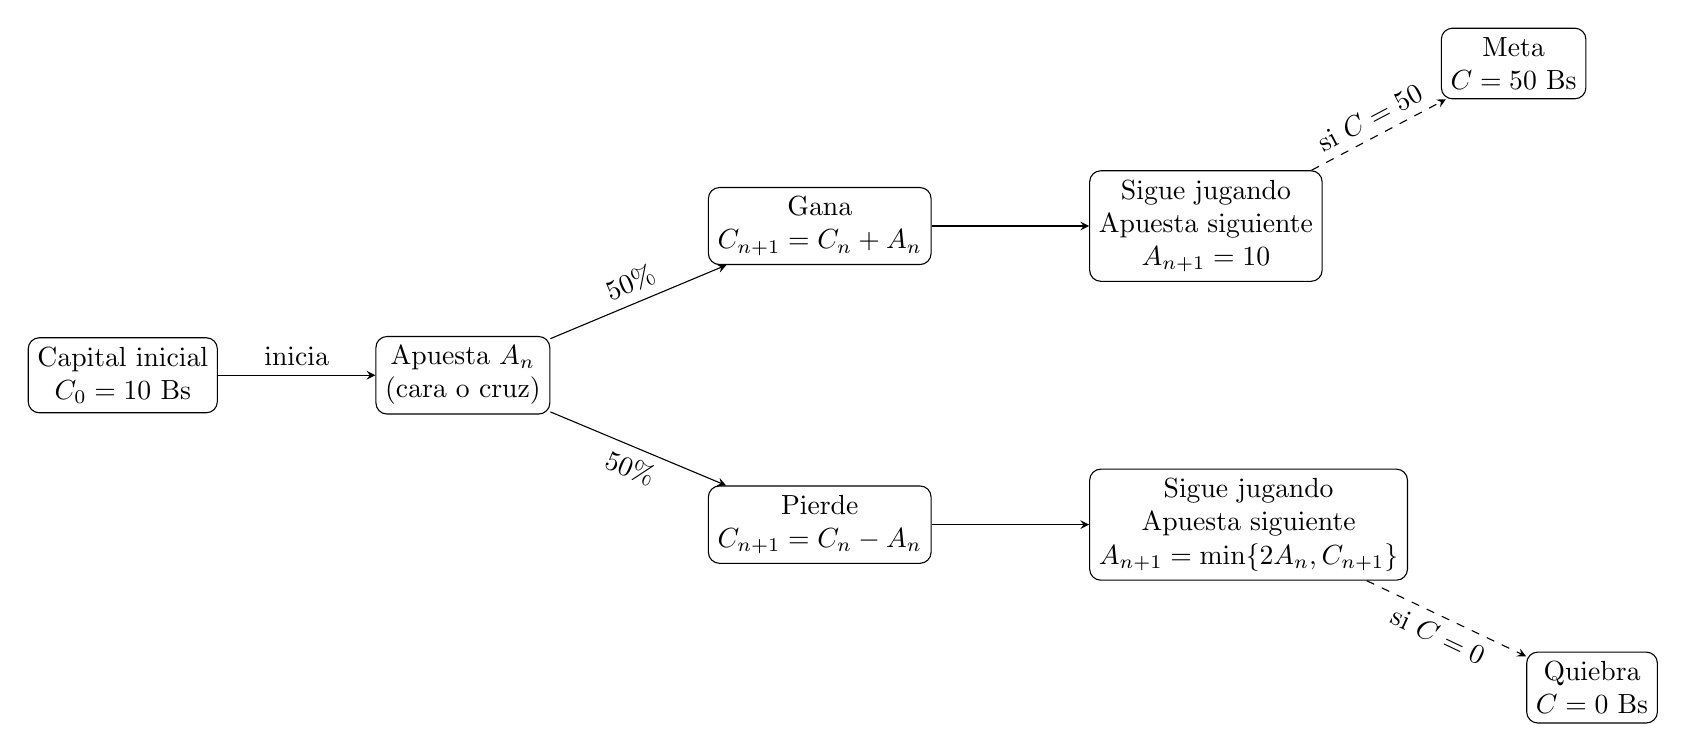
\begin{tikzpicture}[>=stealth, node distance=2.3cm]
  % Nodo jugador inicial
  \node[draw, rounded corners, align=center] (start) {Capital inicial\\$C_0 = 10$ Bs};

  % Nodo apuesta
  \node[draw, rounded corners, right=2.0cm of start, align=center] (bet) {Apuesta $A_n$\\(cara o cruz)};

  % Nodos resultado
  \node[draw, rounded corners, above right=0.9cm and 2.0cm of bet, align=center] (win) {Gana\\$C_{n+1}=C_n + A_n$};
  \node[draw, rounded corners, below right=0.9cm and 2.0cm of bet, align=center] (lose) {Pierde\\$C_{n+1}=C_n - A_n$};

  % Nodos siguientes estados
  \node[draw, rounded corners, right=2.0cm of win, align=center] (afterwin) {Sigue jugando\\Apuesta siguiente\\$A_{n+1}=10$};
  \node[draw, rounded corners, right=2.0cm of lose, align=center] (afterlose) {Sigue jugando\\Apuesta siguiente\\$A_{n+1}=\min\{2A_n,C_{n+1}\}$};

  % Estados meta y quiebra
  \node[draw, rounded corners, above right=0.9cm and 1.5cm of afterwin, align=center] (meta) {Meta\\$C=50$ Bs};
  \node[draw, rounded corners, below right=0.9cm and 1.5cm of afterlose, align=center] (ruina) {Quiebra\\$C=0$ Bs};

  % Flechas
  \draw[->] (start) -- node[above]{inicia} (bet);
  \draw[->] (bet) -- node[above, sloped]{50\%} (win);
  \draw[->] (bet) -- node[below, sloped]{50\%} (lose);
  \draw[->] (win) -- (afterwin);
  \draw[->] (lose) -- (afterlose);

  % Flechas hacia estados absorbentes (conceptuales)
  \draw[->, dashed] (afterwin) -- node[above, sloped]{si $C=50$} (meta);
  \draw[->, dashed] (afterlose) -- node[below, sloped]{si $C=0$} (ruina);
\end{tikzpicture}%
}
\caption{Esquema simplificado del juego de volados con estrategia de duplicación de apuesta.}
\label{fig:volados-esquema}
\end{figure}

\begin{figure}[h]
    \includegraphics[width=1\textwidth]{c1.png}
    \caption{Ejecución del Ejercicio 1 con n=10,30,50}
\end{figure}

\begin{figure}[h]
    \includegraphics[width=1\textwidth]{c1_2.png}
    \caption{Ejecución del Ejercicio 1 con n=100,300,500,1000}
\end{figure}
\hfill\break
\hfill\break
\hfill\break
\hfill\break
\hfill\break
\hfill\break
\hfill\break
\hfill\break
\hfill\break
\hfill\break
\subsection{Camión transportador: probabilidad de exceder la capacidad}
Se analiza el problema de un camión que transporta diariamente cinco tinas de baño. El peso de cada tina es una variable aleatoria continua que se modela mediante una distribución triangular en el intervalo $[190,230]$ kg, con media en $210$ kg. Esto significa que los pesos muy bajos y muy altos son poco probables, mientras que los valores cercanos a $210$ kg tienen mayor probabilidad de ocurrencia.
\hfill\break
\hfill\break
En cada corrida de simulación se generan cinco pesos independientes $X_1,\dots,X_5$ con esa distribución y se calcula la suma total
\[
S = X_1 + X_2 + X_3 + X_4 + X_5.
\]
El camión tiene una capacidad máxima de $1000$ kg, por lo que interesa estimar la probabilidad de que la carga no exceda dicha capacidad, es decir, la probabilidad de que $S \le 1000$. En la simulación se repite el experimento un número grande de veces y se contabiliza la proporción de corridas en las que la suma de los cinco pesos se mantiene dentro del límite permitido.
\hfill\break
\hfill\break
La fracción de veces en que $S \le 1000$ se interpreta como una estimación de la probabilidad verdadera de no sobrecargar el camión. Este valor puede compararse con la aproximación analítica obtenida mediante el teorema del límite central, que modela la distribución de $S$ como aproximadamente normal a partir de la media y la varianza de una tina individual.


\begin{figure}[h]
    \includegraphics[width=0.9\textwidth]{c2.png}
    \caption{Ejecución del Ejercicio 2 con n=10,30,50,100,300,500,1000}
\end{figure}

\hfill\break
\hfill\break

\subsection{Estimación de \texorpdfstring{$\pi$}{pi} mediante simulación}
Se aborda un experimento clásico de Monte Carlo para estimar el valor de $\pi$. La idea se basa en la relación geométrica entre el área de un cuarto de círculo de radio $1$ y el área de un cuadrado de lado $1$. El área del cuarto de círculo es $\pi/4$, mientras que el área del cuadrado es $1$, de modo que la probabilidad de que un punto elegido al azar dentro del cuadrado caiga dentro del cuarto de círculo es
\[
P(\text{punto en el cuarto de círculo}) = \frac{\pi}{4}.
\]
\hfill\break
\hfill\break
El procedimiento consiste en generar puntos $(R_1,R_2)$ uniformemente distribuidos en el cuadrado unitario y verificar cuántos de ellos satisfacen $R_1^2 + R_2^2 \le 1$, condición que caracteriza a los puntos dentro del cuarto de círculo. Si después de $n$ lanzamientos $x$ puntos caen en la región curva, la proporción $x/n$ aproxima la probabilidad anterior, por lo que se puede construir el estimador
\[
\hat{\pi} = 4\frac{x}{n}.
\]
A medida que se incrementa el número de corridas, el valor de $\hat{\pi}$ tiende a estabilizarse alrededor de la constante real, ilustrando de manera sencilla cómo la simulación puede usarse para aproximar cantidades matemáticas difíciles de obtener por métodos directos.

\begin{figure}[h]
    \includegraphics[width=0.9\textwidth]{c3.png}
    \caption{Ejecución del Ejercicio 3 con n=10,30,50,100,300}
\end{figure}


\begin{figure}[h]
    \includegraphics[width=0.9\textwidth]{c3_2.png}
    \caption{Ejecución del Ejercicio 3 con n=500,1000}
\end{figure}

\hfill\break
\hfill\break
\hfill\break
\hfill\break
\hfill\break
\hfill\break
\hfill\break
\hfill\break
\hfill\break
\hfill\break
\hfill\break
\hfill\break
\hfill\break
\subsection{Proyecto de inversión: simulación de la TIR}

Se centra en la evaluación de un proyecto de inversión bajo incertidumbre. El proyecto requiere una inversión fija inicial $AF$ y un capital de trabajo $AC$, cuyos valores no son deterministas sino que se representan mediante distribuciones triangulares con valores pesimistas, más probables y optimistas. De forma similar, los ingresos anuales durante cinco años y las tasas de inflación de cada periodo también se modelan con distribuciones triangulares, reflejando distintos escenarios económicos.
\hfill\break
\hfill\break
Con estos elementos se construyen, para cada año $t$, los flujos de caja nominales, considerando ingresos, costos, depreciación y el efecto de los impuestos. Luego se corrigen por la inflación acumulada para obtener flujos reales $S_t$. Además, al final del quinto año se incluye un valor de rescate $VR$ asociado a la recuperación parcial de la inversión.
\hfill\break
\hfill\break
La rentabilidad del proyecto se resume mediante la \textit{tasa interna de retorno} (TIR), definida como el valor $r$ que satisface la ecuación
\[
\sum_{t=1}^{5} \frac{S_t}{(1+r)^t} + \frac{VR}{(1+r)^5} - AF - AC = 0.
\]
Para cada escenario simulado se resuelve numéricamente esta ecuación y se obtiene un valor de TIR. Repitiendo el proceso muchas veces se genera una muestra de posibles tasas internas, a partir de la cual se puede estimar la probabilidad de que la TIR supere una tasa mínima de aceptación (TREMA), así como analizar la forma de la distribución acumulada de la rentabilidad del proyecto.

\begin{figure}[h]
    \includegraphics[width=0.9\textwidth]{c4.png}
    \caption{Ejecución del Ejercicio 4 con n=10,30,50,100,300}
\end{figure}

\begin{figure}[h]
    \includegraphics[width=0.8\textwidth]{c4_2.png}
    \caption{Ejecución del Ejercicio 4 con n=500,1000}
\end{figure}

\hfill\break
\hfill\break
\hfill\break
\hfill\break
\hfill\break
\hfill\break
\hfill\break
\hfill\break
\hfill\break
\hfill\break
\hfill\break
\hfill\break
\hfill\break
\hfill\break
\hfill\break
\hfill\break
\hfill\break
\hfill\break
\hfill\break
\hfill\break
\hfill\break
\hfill\break
\hfill\break
\hfill\break
\subsection{Modelo de inventarios \texorpdfstring{$(q,R)$}{(q,R)}}

Se estudia un sistema de inventarios gestionado mediante una política de reorden $(q,R)$, donde $q$ representa la cantidad fija que se pide cada vez que se coloca una orden y $R$ es el punto de reorden. El nivel de inventario se revisa al inicio de cada mes. Si el inventario disponible es inferior a $R$, se emite un pedido por $q$ unidades.
\hfill\break
\hfill\break
La demanda mensual del producto se modela como una variable discreta que puede tomar valores entre 35 y 60 unidades, con probabilidades empíricas obtenidas de datos históricos. Para capturar la estacionalidad a lo largo del año, cada demanda base se multiplica por un factor estacional específico del mes, de modo que algunos periodos presentan demanda alta y otros demanda baja. Además, el tiempo de entrega del proveedor es aleatorio y puede ser de 1, 2 o 3 meses con probabilidades dadas, lo que implica que los pedidos realizados hoy pueden llegar en distintos momentos futuros.
\hfill\break
\hfill\break
En cada mes se actualiza el inventario sumando las llegadas pendientes, se genera la demanda estocástica y se decide cuánto se logra satisfacer. Si el inventario no alcanza, se registran faltantes. Al final del horizonte de 12 meses se calculan tres componentes de costo: costo de ordenar (proporcional al número de pedidos emitidos), costo de mantener inventario (proporcional al nivel promedio de existencias) y costo de faltantes (proporcional a las unidades no atendidas). La suma de estos términos da el costo total anual asociado al par $(q,R)$. Repitiendo la simulación para distintos valores de $q$ y $R$ es posible identificar combinaciones que producen costos promedio más bajos y, por tanto, constituyen políticas de inventario casi óptimas.

\begin{figure}[!h]
    \includegraphics[width=0.8\textwidth]{c5.png}
    \caption{Ejecución del Ejercicio 5 con n=10}
\end{figure}

\begin{figure}[!h]
    \includegraphics[width=0.8\textwidth]{c5_2.png}
    \caption{Ejecución del Ejercicio 5 con n=30}
\end{figure}

\begin{figure}[!h]
    \includegraphics[width=0.8\textwidth]{c5_3.png}
    \caption{Ejecución del Ejercicio 5 con n=50}
\end{figure}

\begin{figure}[!h]
    \includegraphics[width=0.8\textwidth]{c5100.png}
    \caption{Ejecución del Ejercicio 5 con n=100}
\end{figure}

\begin{figure}[!h]
    \includegraphics[width=0.8\textwidth]{c5_4.png}
    \caption{Ejecución del Ejercicio 5 con n=300}
\end{figure}


\begin{figure}[!h]
    \includegraphics[width=0.8\textwidth]{c5_5.png}
    \caption{Ejecución del Ejercicio 5 con n=500}
\end{figure}

\begin{figure}[!h]
    \includegraphics[width=0.8\textwidth]{c5_6.png}
    \caption{Ejecución del Ejercicio 5 con n=1000}
\end{figure}


\hfill\break
\hfill\break
\hfill\break
\hfill\break
\hfill\break
\hfill\break
\hfill\break
\hfill\break
\hfill\break
\hfill\break
\hfill\break
\hfill\break
\hfill\break
\hfill\break
\hfill\break
\hfill\break
\hfill\break
\hfill\break
\hfill\break
\hfill\break
\hfill\break
\hfill\break
\hfill\break
\hfill\break
\hfill\break
\hfill\break
\hfill\break
\hfill\break
\hfill\break
\hfill\break
\hfill\break
\hfill\break
\hfill\break
\hfill\break
\hfill\break
\hfill\break
\hfill\break
\hfill\break
\hfill\break
\hfill\break
\hfill\break
\hfill\break
\hfill\break
\hfill\break
\hfill\break
\hfill\break
\hfill\break
\hfill\break
\hfill\break
\hfill\break
\hfill\break
\hfill\break
\hfill\break
\hfill\break
\hfill\break
\hfill\break
\hfill\break
\hfill\break
\hfill\break
\hfill\break
\hfill\break
\hfill\break
\hfill\break
\hfill\break
\hfill\break
\hfill\break
\hfill\break
\hfill\break
\hfill\break
\hfill\break
\hfill\break
\hfill\break
\hfill\break
\hfill\break
\hfill\break
\hfill\break
\hfill\break
\hfill\break
\hfill\break
\hfill\break
\hfill\break
\hfill\break
\hfill\break
\hfill\break
\hfill\break
\hfill\break
\hfill\break
\hfill\break
\hfill\break
\hfill\break
\hfill\break
\hfill\break
\hfill\break
\hfill\break
\hfill\break
\hfill\break
\hfill\break
\hfill\break
\hfill\break
\subsection{Juego 7--11: probabilidad de quiebra}

Se considera el juego de dados conocido como 7--11. En cada partida el jugador lanza dos dados equilibrados y observa la suma de los resultados. Las reglas básicas son:
\begin{itemize}
    \item Si en la primera tirada la suma es 7 u 11, el jugador gana inmediatamente.
    \item Si la suma es 2, 3 o 12, el jugador pierde de forma inmediata.
    \item Si la suma es 4, 5, 6, 8, 9 o 10, ese valor se convierte en el \emph{punto}. A partir de entonces se siguen realizando tiradas hasta que:
    \begin{itemize}
        \item vuelva a salir el punto, en cuyo caso el jugador gana, o
        \item aparezca un 7, en cuyo caso el jugador pierde.
    \end{itemize}
\end{itemize}
Cada partida se puede ver como una variable aleatoria que toma el valor 1 si el jugador gana y 0 si pierde.
\hfill\break
\hfill\break
El problema de interés no es sólo la probabilidad de ganar una partida aislada, sino la \textit{probabilidad de quiebra} cuando el juego se repite muchas veces. Se considera un jugador que comienza con un capital inicial, realiza apuestas unitarias y continúa jugando mientras su capital esté entre 1 y una meta prefijada (por ejemplo, 50 unidades monetarias). En cada partida, si gana aumenta su capital en 1 y si pierde lo disminuye en 1. El proceso termina cuando el capital llega a 0 (quiebra) o alcanza la meta.
\hfill\break
\hfill\break
La simulación repite este esquema muchas veces, registrando en cuántas trayectorias el jugador termina en quiebra. La proporción de trayectorias que terminan en capital cero proporciona una estimación de la probabilidad de ruina para las condiciones iniciales consideradas, lo que permite evaluar el riesgo asociado a seguir jugando bajo estas reglas.


\begin{figure}[!h]
    \includegraphics[width=0.9\textwidth]{c6.png}
    \caption{Ejecución del Ejercicio 6 con n=10,30,50,100,300,500,1000}
\end{figure}



\hfill\break
\hfill\break
\hfill\break
\hfill\break

\section{Resultados y análisis}
\subsection*{Juego de volados}

Las gráficas de convergencia muestran que para $n$ pequeño (por ejemplo, $10$ o $30$ corridas) la estimación de la probabilidad de alcanzar la meta presenta oscilaciones importantes, lo que refleja la alta variabilidad inherente a pocas partidas. A medida que $n$ aumenta (500, 1000 y en especial 3000 o 5000), la proporción acumulada de éxitos tiende a estabilizarse alrededor de un valor cercano a la probabilidad teórica mencionada en el texto. Esto ilustra claramente la ley de los grandes números: el promedio muestral converge hacia la verdadera probabilidad del evento.

\begin{figure}[!h]
    \includegraphics[width=0.8\textwidth]{h1bajo.png}
    \caption{Histograma del Ejercicio 1 con un numero de corridas pequeño}
\end{figure}

\begin{figure}[!h]
    \includegraphics[width=0.8\textwidth]{h1alto.png}
    \caption{Histograma del Ejercicio 1 con un numero de corridas grande}
\end{figure}

\hfill\break
\hfill\break
\hfill\break
\hfill\break

\subsection*{Camión transportador}

La probabilidad experimental de que la suma de los pesos no exceda la capacidad del camión se aproxima a un valor muy cercano al esperado analíticamente. Para corridas pequeñas pueden observarse porcentajes algo alejados de $0.9969$, pero al aumentar el número de simulaciones la estimación converge y la diferencia con el valor teórico se reduce significativamente. Esto confirma que el generador de pesos triangulares y el algoritmo de simulación están implementados correctamente.


\begin{figure}[!h]
    \includegraphics[width=0.8\textwidth]{h2bajo.png}
    \caption{Histograma del Ejercicio 2 con un numero de corridas pequeño}
\end{figure}

\begin{figure}[!h]
    \includegraphics[width=0.8\textwidth]{h2alto.png}
    \caption{Histograma del Ejercicio 2 con un numero de corridas grande}
\end{figure}


\subsection*{Estimación de \texorpdfstring{$\pi$}{pi}}

En el experimento geométrico, la sucesión de estimadores $\hat{\pi}_k$ presenta al inicio una alta variabilidad, con valores que pueden estar alejados del número $\pi$. No obstante, para $n$ de orden miles, la curva se ``aplana'' en torno a $3.14$, y la diferencia absoluta entre el estimador final y el valor real se vuelve pequeña. La gráfica con la línea de referencia en $\pi$ permite apreciar visualmente la convergencia. Este resultado pone de manifiesto la potencia del método de Monte Carlo para aproximar constantes matemáticas a partir de consideraciones probabilísticas simples.


\begin{figure}[!h]
    \includegraphics[width=0.8\textwidth]{h3bajo.png}
    \caption{Histograma del Ejercicio 3 con un numero de corridas pequeño}
\end{figure}

\begin{figure}[!h]
    \includegraphics[width=0.8\textwidth]{h3alto.png}
    \caption{Histograma del Ejercicio 3 con un numero de corridas grande}
\end{figure}


\subsection*{Proyecto de inversión}

La simulación del proyecto de inversión genera una distribución de valores de TIR que refleja la incertidumbre en los costos iniciales, los ingresos anuales y las tasas de inflación. En general, se observa que la TIR puede variar en un rango amplio, incluso tomando valores inferiores a la TREMA en algunos escenarios pesimistas. La función \texttt{ejercicio4()} calcula la proporción de corridas en las que la TIR supera la tasa mínima, lo que puede interpretarse como una estimación de la probabilidad de que el proyecto sea aceptable desde el punto de vista financiero. El histograma y la distribución acumulada empírica permiten analizar el riesgo con mayor detalle, mostrando, por ejemplo, percentiles de la TIR y la concentración de probabilidad alrededor de ciertos valores.

\begin{figure}[!h]
    \includegraphics[width=0.8\textwidth]{h4bajo.png}
    \caption{Histograma del Ejercicio 4 con un numero de corridas pequeño}
\end{figure}

\begin{figure}[!h]
    \includegraphics[width=0.8\textwidth]{h4alto.png}
    \caption{Histograma del Ejercicio 4 con un numero de corridas grande}
\end{figure}




\subsection*{Modelo de inventarios}

En el sistema de inventarios, la tabla de costos promedio obtenida al recorrer distintos valores de $(q,R)$ permite identificar combinaciones que producen costos anuales menores. Los mapas de calor muestran regiones claras donde el costo es relativamente bajo, rodeadas por zonas donde el costo aumenta debido a excesivos faltantes o a inventarios demasiado grandes. El análisis visual facilita la selección de un par $(q,R)$ cercano al óptimo, sin necesidad de derivar fórmulas complicadas de costo esperado. Además, al repetir las simulaciones para varios tamaños de muestra se observa que los costos promedio estimados tienden a estabilizarse, lo cual respalda la confiabilidad de las conclusiones.


\begin{figure}[!h]
    \includegraphics[width=0.8\textwidth]{ed5bajo.png}
    \caption{Gráfico 3D del Ejercicio 5 con un numero de corridas pequeño}
\end{figure}

\begin{figure}[!h]
    \includegraphics[width=0.8\textwidth]{calor5bajo.png}
    \caption{Mapa de calor del Ejercicio 5 con un numero de corridas pequeño}
\end{figure}

\begin{figure}[!h]
    \includegraphics[width=0.8\textwidth]{3d5alto.png}
    \caption{Gráfico 3D del Ejercicio 5 con un numero de corridas grande}
\end{figure}

\begin{figure}[!h]
    \includegraphics[width=0.8\textwidth]{calor5alto.png}
    \caption{Mapa de calor del Ejercicio 5 con un numero de corridas grande}
\end{figure}



\subsection*{Juego 7--11}

En el juego 7--11, la gráfica de probabilidad de quiebra acumulada muestra nuevamente oscilaciones iniciales que se reducen al aumentar el número de corridas. Dependiendo de las probabilidades de ganar cada juego y de los límites de capital elegidos (0 y 50), la probabilidad de ruina puede ser relativamente alta o moderada, pero la simulación permite cuantificarla numéricamente sin necesidad de resolver explícitamente el modelo de ruina del jugador. Este resultado sirve como advertencia sobre la persistencia en juegos de azar: aun cuando la probabilidad de ganar una partida individual no parezca desfavorable, la repetición sucesiva con un capital finito termina llevando con frecuencia a la quiebra.


\begin{figure}[!h]
    \includegraphics[width=0.8\textwidth]{h6bajo.png}
    \caption{Histograma del Ejercicio 6 con un numero de corridas pequeño}
\end{figure}

\begin{figure}[!h]
    \includegraphics[width=0.8\textwidth]{h6alto.png}
    \caption{Histograma del Ejercicio 6 con un numero de corridas grande}
\end{figure}


\section{Conclusiones}

\begin{itemize}
    \item El uso de un generador congruencial mixto como fuente de números pseudoaleatorios permite construir modelos de simulación versátiles para una amplia variedad de sistemas, desde juegos de azar hasta inventarios y proyectos de inversión. La correcta implementación del generador es fundamental para garantizar la calidad estadística de los resultados.
    \hfill\break
    \item La simulación por computadora facilita la solución de problemas donde el análisis exacto es difícil o tedioso. En el caso del camión transportador y la estimación de $\pi$, fue posible comparar las estimaciones de Monte Carlo con resultados analíticos aproximados, observando una excelente concordancia a medida que aumentó el número de corridas.
    \hfill\break
    \item En aplicaciones como el proyecto de inversión y el sistema de inventarios, la simulación proporciona información que sería muy complicada de obtener con métodos puramente analíticos. La distribución de la TIR y el costo esperado bajo distintas políticas $(q,R)$ se derivan de manera natural a partir de las corridas simuladas, lo que ayuda a evaluar el riesgo y a tomar decisiones más informadas.
    \hfill\break
    \item Los juegos de volados y 7--11 ilustran claramente la noción de ruina del jugador y la importancia de considerar el capital disponible y las metas de ganancia. Las simulaciones muestran que, aun en juegos aparentemente justos, la probabilidad de alcanzar la meta puede ser limitada y la probabilidad de quiebra considerable cuando se repiten las apuestas muchas veces.
    \hfill\break
    \item En conjunto, los seis ejemplos analizados demuestran que la simulación de sistemas no sólo es una herramienta teórica, sino una metodología práctica para explorar el comportamiento de modelos estocásticos, estimar probabilidades, analizar costos y evaluar alternativas de decisión en contextos reales.
\end{itemize}

\section{Bibliografía}
\begin{thebibliography}{99}

\bibitem{cossbu}
Coss Bu, R. (2010). \textit{Simulación: un enfoque práctico}. McGraw--Hill.

\bibitem{law}
Law, A. M. (2015). \textit{Simulation Modeling and Analysis} (5th ed.). McGraw--Hill.

\bibitem{ross}
Ross, S. M. (2013). \textit{Simulation} (5th ed.). Academic Press.

\bibitem{banks}
Banks, J.; Carson, J. S.; Nelson, B. L.; Nicol, D. M. (2010). \textit{Discrete-Event System Simulation} (5th ed.). Pearson.

\bibitem{devroye}
Devroye, L. (1986). \textit{Non-Uniform Random Variate Generation}. Springer.

\bibitem{pidd}
Pidd, M. (2004). \textit{Computer Simulation in Management Science} (5th ed.). John Wiley \& Sons.

\end{thebibliography}

\end{document}
